
\chapter[Unbalanced Co-Optimal Transport]{Unbalanced Co-Optimal Transport}

\localtableofcontents*

\chaptermark{\textbf{Unbalanced Co-Optimal Transport}}

This chapter presents the results from the paper \citep{Tran23} and addresses the unbalaced extension
of Co-Optimal transport.
Optimal transport (OT) compares probability distributions by computing a meaningful alignment
between their samples. Co-optimal transport (COOT) takes this comparison further
by inferring an alignment between features as well. While this approach leads to
better alignments and generalizes both OT and Gromov-Wasserstein distances,
we provide a theoretical result showing that it is sensitive to outliers
that are omnipresent in real-world data. This prompts us to propose unbalanced COOT
for which we provably show its robustness to noise in the compared datasets.
To the best of our knowledge, this is the first such result for OT methods in incomparable spaces.
With this result in hand, we provide empirical evidence of this robustness
for the challenging tasks of heterogeneous domain adaptation with and without
varying proportions of classes and simultaneous alignment of samples and features across
single-cell measurements.

%%%%%%%%%%%%%%%%%%%%%%%%%%%%%%%%%%%%%%%%%%%%%%
\section{Introduction}
%%%%%%%%%%%%%%%%%%%%%%%%%%%%%%%%%%%%%%%%%%%%%%

The last decade has witnessed many successful applications of optimal
transport (OT) \citep{Monge81,Kanto42} in machine learning, namely in domain adaptation \citep{Courty16}, generative adversarial networks \citep{Arjovsky17},
classification \citep{Frogner15}, dictionary learning \citep{Rolet16},
semi-supervised learning \citep{Solomon14}. When the
supports of the probability measures lie in the same ground metric space, it is natural to use the distance defined by the metric
to induce the cost, which leads to the famous Wasserstein distance \citep{Villani03}. When they do not, one can rely on the idea of Gromov-Hausdorff distance \citep{Gromov81} and its equivalent reformulations \citep{Gromov99,Kalton99,Burago01}, and adapt them to the setting of metric measure spaces \citep{Gromov99}. This results in, for example, the Gromov-Wasserstein
(GW) distance \citep{Memoli07,Memoli11,Sturm12}, which has been widely used in many applications, namely in shape matching \citep{Memoli11},
comparing kernel matrices \citep{Peyre16}, graphs \citep{Vayer19b,Xu19,Xu19b},
computational biology \citep{Demetci22}, heterogeneous domain adaptation \citep{Yan18},
correspondence alignment \citep{Solomon16}, machine translation \citep{Melis18}.

By construction, the GW distance can only provide the sample alignment that best preserves the intrinsic geometry of the distributions and, as such, compares square pairwise relationship matrices. The CO-Optimal transport (COOT) \citep{Redko20,Chowdhury21b} goes beyond these limits by simultaneously learning two independent (feature and sample) correspondences, and thus provides greater flexibility over the GW distance in terms of usage and interpretability. First, it allows us to measure similarity between arbitrary-size matrices. An interesting use case is, for instance, on tabular data, which are usually expressed as a matrix whose rows represent samples and columns represent features. For the GW distance,
the similarity or distance matrix (or any square matrix derived from the data)
must be calculated in advance and the effect of the individual variables is lost during this computation. On the other hand, COOT can bypass this step as it can use either the tabular data directly or the similarity matrices as inputs. Second, COOT provides both sample and feature correspondences. These feature correspondences are also interpretable and allow to recover relations between the features of two different datasets even when they do not lie in the same space.

Similar to classical OT, COOT enforces hard constraints on the marginal distributions
both between samples and features. These constraints lead to two main limitations:
(1) imbalanced datasets where samples or features are re-weighted
cannot be accurately compared; (2) mass transportation \emph{must} be exhaustive:
outliers, if any, must be matched regardless of the cost they induce.
To circumvent these limitations, we propose to relax the mass preservation constraints
in the COOT distance and study a broadly applicable and general OT framework
that includes several well-studied cases presented in \Cref{t:ucoot_comparisons}.

\paragraph{Related work.}
To relax the OT marginal constraints, a straightforward solution is to control
the difference between the marginal distributions of the transportation plan
and the data by some discrepancy measure, e.g., Kullback-Leibler divergence.
In classical OT, this gives rise to the unbalanced OT (UOT),
which was first proposed by~\citep{Benamou03}.
The theoretical and numerical aspects of this extension
have been studied extensively \citep{Liero18,Chizat18b,Chizat18a,Khiem20}
and are gaining increasing attention in the machine
learning community, with wide-range applications, namely in
domain adaptation \citep{Fatras21}, generative adversarial networks
\citep{Balaji20, Yang19}, dynamic tracking \citep{Lee19}, crowd counting \citep{Ma21},
neuroscience \citep{janati2019group, bazeille2019} or
modeling cell developmental trajectories \citep{Schiebinger19}.

Unbalanced OT and its variants are usually sought for
their known robustness to outliers \citep{Mukherjee21,Balaji20,Fatras21}.
This appealing property goes beyond classical OT. For instance,
to compare signed and non-negative measures in incomparable spaces,
unbalanced OT \citep{Liero18} can be blended with the
$L_p$-transportation distance \citep{Sturm06}, which leads to the
Sturm-Entropic-Transport distance \citep{Ponti20}, or with the GW distance,
which gives rise to the unbalanced GW (UGW) distance \citep{Sejourne20}.
Also motivated by the unbalanced OT, \citep{Zhang21} proposed a relaxation of the
bidirectional Gromov-Monge distance called unbalanced bidirectional Gromov-Monge divergence.
\begin{table}[t]
  \small
	\centering
  \begin{tabular}{l *4c}
    \toprule
    & Across spaces & Sample alignment & Feature alignment & \makecell{Robust to outliers} \\
    \midrule
    OT & \nomark & \yesmark & \nomark & \nomark \citep{Fatras21} \\
    UOT & \nomark & \yesmark & \nomark & \yesmark \citep{Fatras21} \\
    GW & \yesmark & \yesmark & \nomark & \nomark (Prop. \ref{prop:coot_not_robust}) \\
    UGW & \yesmark & \yesmark & \nomark & \yesmark (Thm. \ref{thm:ucoot_robust}) \\
    COOT & \yesmark & \yesmark & \yesmark & \nomark (Prop. \ref{prop:coot_not_robust}) \\
    UCOOT & \yesmark & \yesmark & \yesmark & \yesmark (Thm. \ref{thm:ucoot_robust}) \\
    \bottomrule
    \hline
  \end{tabular}
  \caption{Properties of different OT formulations generalized by UCOOT.
  The proposed UCOOT is not only able to learn informative feature alignments,
  but also robust to outliers.
  \label{t:ucoot_comparisons}}
\end{table}

\paragraph{Contributions.} In this work, we introduce an unbalanced extension of COOT
called ``Unbalanced CO-Optimal transport'' (UCOOT). UCOOT -- defined for both discrete and
continuous data -- is a general framework that encompasses all the OT variants displayed
in \Cref{t:ucoot_comparisons}. Our main contribution is to show that UCOOT is provably robust
to both samples and features outliers, while its balanced counterpart can be made
arbitrarily large with strong enough perturbations. To the best of our knowledge,
this is the first time such a general robustness result is established for OT across different spaces.
Our theoretical findings are showcased in unsupervised heterogeneous domain adaptation
and single-cell multi-omic data alignment, demonstrating a very competitive performance.

\paragraph{Notations.} For any integer $n \geq 1$, we write $[n] := \{1,...,n\}$.
Given a Polish space $X$, we denote $\cM^+(X)$ the set of nonnegative and finite Borel
measures over $X$. For any $\mu \in \cM^+(X)$, we denote
its mass by $m(\mu) := \mu(X)$.
Unless specified otherwise, we always consider fully supported measures,
i.e. $\text{supp}(\mu) = X$, for any measure $\mu \in \cM^+(X)$.
The product measure of two measures $\mu$ and $\nu$ is defined as:
$d (\mu \otimes \nu)(x,y) := d\mu(x) d\nu(y)$.
Given $\pi \in \cM^{+}(X \times Y)$, we denote
$(\pi_{\#1}, \pi_{\#2})$ its marginal distributions i.e. $d\pi_{\#1} = \int_{Y} d\pi$ and
$d\pi_{\#2} = \int_{X} d\pi$.
For $\mu, \nu \in \cM^+(X)$, the Kullback-Leibler divergence is defined by
$\kl(\mu|\nu) := \int \frac{d \mu}{ d \nu} \log \frac{d \mu}{ d \nu} \mathrm d\nu
- \int \mathrm d\mu + \int \mathrm d\nu$ if $\mu \ll \nu$ and set to $+\infty$ otherwise.
Finally, the indicator divergence $\iota_{=}(\mu | \nu)$ is equal to 0 if $\mu = \nu$
and $+\infty$ otherwise.

%%%%%%%%%%%%%%%%%%%%%%%%%%%%%%%%%%%%%%%%%%%%%%%%%%

%%%%%%%%%%%%%%%%%%%%%%%%%%%%%%%%%%%%%%%%%%%%%%%
\section{From COOT to Unbalanced Co-Optimal Transport} \label{sec:ucoot}
The ultimate goal behind the CO-Optimal Transport (COOT)
framework is the simultaneous alignment of samples \emph{and} features to allow for
comparisons across spaces of different dimensions. In this section, we discuss
OT formulations including OT, UOT, GW, UGW and COOT, then introduce the proposed UCOOT
and show how the aforementioned distances fall into our framework.

% \iffalse After some examples, we present our main theoretical contribution:the robustness to sample and feature outliers. \fi

\paragraph{From sample alignment to sample-feature alignment.}
Let $(X_1^s, \mu_1^s)$ and $(X_2^s, \mu_2^s)$ be a pair of compact measure spaces such that
$X_1^s$ and $X_2^s$ belong to some common metric space $(\cE, d)$.
Classical (unbalanced) optimal transport infers one alignment (or joint distribution)
$\pi^s \in \cM^+(X_1^{s} \times X_2^s)$ with marginals $(\pi^{s}_{\#1}, \pi^{s}_{\#2})$
close to $(\mu_1^s, \mu_2^s)$ according to some appropriate divergence $D$ such that
the cost $\int c(x_1, x_2) \; \mathrm d\pi^{s}(x_1, x_2) + D(\pi^{s}_{\#1} | \mu_1^s)
+ D(\pi^{s}_{\#2} | \mu_2^s)$ is minimal. For instance, in balanced (resp. unbalanced) OT,
$D$ corresponds to the indicator divergence (resp. KL divergence or TV).
To define a generalized OT beyond one single alignment, we must first introduce
a new pair of measure spaces $(X_1^{f}, \mu_1^f)$ and $(X_2^{f}, \mu_2^f)$.
Intuitively,  the two transport plans that must be inferred: $\pi^s$ across \emph{samples}
and $\pi^f$ across \emph{features}, must minimize a cost of the form
$\iint c((x_1^s, x_1^f), (x_2^s, x_2^f)) \; \mathrm d\pi^s(x_1^s, x_2^s)\; \mathrm d \pi^f(x_1^f, x_2^f)$
where $c((x_1^s, x_1^f), (x_2^s, x_2^f))$ is the \emph{joint} cost of aligning
the sample-feature pairs $(x_1^s, x_1^f)$ and $(x_2^s, x_2^f)$.

However, unlike OT,
there is no underlying ambient metric space in which comparisons between these pairs
are straightforward. Thus, we consider a simplified cost of the form:
$c((x_1^s, x_1^f), (x_2^s, x_2^f)) = |\xi_1(x_1^s, x_1^f) - \xi_2(x_2^s, x_2^f)|^p$, for $p \geq 1$
and some scalar functions $\xi_1, \xi_2$ that define the sample-feature interactions.
A similar definition was adopted by~\citep{Chowdhury21b} to extend COOT to the continuous setting
in the context of hypergraphs. Formally, our general formulation takes
pairs of \emph{sample-feature spaces} defined as follows.

\begin{definition}[Sample-feature space]
Let $(X^s, \mu^s)$ and $(X^f, \mu^f)$ be compact Polish measure spaces, where $\mu^f \in \cM^+(X^f)$
and $\mu^s \in \cM^+(X^s)$. Let $\xi$ be a scalar integrable function in
$L^p(X^s \times X^f, \mu^s \otimes \mu^f)$. We call the triplet
$\cX = ((X^s, \mu^s), (X^f, \mu^f), \xi)$ a sample-feature space and $\xi$ is called an interaction.
\end{definition}
%
%%%%%%%%%%%%%%%%%%%%%%%%%%%%%%%%%%%%%%%%%%%%%%%%
\begin{definition}[Generalized COOT]
\label{def:ucoot}
Given two divergences $D_1$ and $D_2$, we define the generalized COOT of order $p$
between $\mathbb{X}_1 = ((X_1^s, \mu_1^s), (X_1^f, \mu_1^f), \xi_1)$ and
$\mathbb{X}_2 = ((X_2^s, \mu_2^s), (X_2^f, \mu_2^f), \xi_2)$ by:
\begin{equation}
\label{eq:ucoot}
  \begin{split}
  \inf_{\substack{\pi^s \in \cM^+(X_1^s \times X_2^s) \\
  \pi^f \in \cM^+(X_1^f \times X_2^f) \\ m(\pi^s) = m(\pi^f)}}
  &\underbrace{\iint |\xi_1(x_1^s, x_1^f) - \xi_2(x_2^s, x_2^f)|^p
  \; \mathrm d\pi^s \; \mathrm d \pi^f}_{\text{transport cost of sample-feature pairs}}
  + \underbrace{\sum_{k=1}^2\lambda_k D_k(\pi^s_{\#k} \otimes \pi^f_{\#k} |
  \mu^s_k \otimes \mu^f_k)}_{\text{mass destruction / creation penalty}},
  \end{split}
\end{equation}
for $\lambda_1, \lambda_2 >0$ and $p \geq 1$.
\end{definition}
As the multiplicative nature between $\pi^s$ and $\pi^f$ leads to an invariance by the scaling map
$\alpha \mapsto (\alpha \pi^s, \frac{1}{\alpha} \pi^f)$, for $\alpha > 0$,
we further impose the equal mass constraint $m(\pi^s) = m(\pi^f)$.

It is worth mentioning that Formulation \eqref{eq:ucoot} is not the only way to
relax the marginal constraints. For example, instead of
$D_k(\pi^s_{\#k} \otimes \pi^f_{\#k} | \mu^s_k \otimes \mu^f_k)$,
one can consider $D_k(\pi^s_{\#k} | \mu^s_k) + D_k( \pi^f_{\#k} | \mu^f_k)$,
or $D_s(\pi^s_{\#1} \otimes \pi^s_{\#2} | \mu^s_1 \otimes \mu^s_2)$,
for some divergence $D_s$. However, amongst these choices,
ours is the only one which can be recast as a variation of the unbalanced OT problem.
This allows us to leverage the known techniques in unbalanced OT to justify
the theoritical and practical properties, namely \Cref{prop:existence}
and \Cref{thm:ucoot_robust} below.

Note that the problem above is very general and can, with some additional
constraints, recover exact OT, UOT, GW, UGW, COOT (see \Cref{t:examples}).
In particular, if the measures $(\mu^s_1, \mu^s_2)$ and $(\mu^f_1, \mu^f_2)$
are probability measures, then setting $D_1 = D_2 = \iota_=$ leads to the
COOT problem first introduced in the discrete case in \citep{Redko20} and
recently generalized to the continuous setting in \citep{Chowdhury21b}
\footnote{Note that, \citep{Chowdhury21b} consider \textbf{bounded measurable} function
on the Polish measure space, whereas we work with \textbf{integrable} function
on the \textbf{compact} Polish measure space.}
In this work, we relax the hard constraints and consider a more flexible formulation
with the KL divergence:
\begin{definition}[UCOOT]
   We define Unbalanced COOT ($\ucoot$) as in \Cref{eq:ucoot} with $D_1 = D_2 = \kl$.
   We write $\ucoot_{\lambda}(\cX_1, \cX_2)$ to indicate the UCOOT between
   two sample-feature spaces $\cX_1$ and $\cX_2$, for a given
   pair of hyperparameters $\lambda = (\lambda_1, \lambda_2)$.
\end{definition}
While various properties of the divergences $D_k$ have been extensively studied
in the context of unbalanced OT by several authors \citep{Chizat17,Frogner15},
the concept of sample-feature interaction requires more clarification.
Let us consider some simple examples.
In the discrete case, we consider $n$ observations of $d$ features
represented by matrix $A \in \bbR^{n \times d}$. In this case, the space $X^s$ (resp. $X^f$)
is not explicitly known but can be characterized by the finite set $[n]$ (resp. $[d]$),
up to an isomorphism. Assuming that all samples (resp. features) are equally important,
the discrete empirical measures can be given by uniform weights $\mu^s = \frac{1_{n}}{n}$
(resp. $\mu^f = \frac{1_{d}}{d}$). The most natural sample-feature interaction $\xi$ is simply
the index function $\xi(i, j) = A_{ij}$. In the continuous case,
we assume that data stream from a continuous random variable $a \sim \mu_s \in \cP(\bbR^d)$
for which an interaction function can be $\xi(a, j) = a_j$.
\begin{table}[t]
  \centering
  \small
  \begin{tabular}{l *4c}
      \toprule
          & Shape of inputs & Coupling constraint & Scalar function & Divergence \\
      \midrule
      OT   & $d_1 = d_2$              & $\pi^f = I_{d_1} = I_{d_2}$ & $\xi(i, j) = A_{ij}$                        & $\iota_=$ \\
      GW   & $n_1 = d_1$, $n_2 = d_2$ & $\pi^f = \pi^s$             & $\xi(i, j) = \text{dist}( A_{i.}, A_{j.} )$ & $\iota_=$ \\
      COOT & --                       & --                          & $\xi(i, j) = A_{ij}$                        & $\iota_=$ \\
      semi-d. COOT & --               & --                          & $\xi(a, j) = a_j$                           & $\iota_=$ \\
      UCOOT & --                      & --                          & $\xi(i, j) = A_{ij}$                        & KL \\
        \bottomrule
        \hline
        \end{tabular}
        \caption{Conditions under which different OT formulations fall within
        the generalized framework of \Cref{def:ucoot}.
        ``semi-d'' refers to ``semi-discrete'' setting, where
        $\mu_s$ is a continuous probability and $\mu_d = 1_d/d$.
        Here, $I_d$ is the identity matrix in $\bbR^d$.
  \label{t:examples}}
\end{table}
\begin{proposition} \label{prop:existence}
For any $D_1$, $D_2 \in \{ \iota_{=}, \kl \}$, Problem \eqref{def:ucoot} (in Equation \eqref{eq:ucoot})
admits a minimizer.
\end{proposition}

\begin{remark}
The existence of minimizer shown in \Cref{prop:existence}
can be extended to a larger family of Csiszár divergences \citep{Csiszar63}.
A general proof is given in the Appendix.
\end{remark}

\paragraph{Relation between UCOOT and COOT.} When $ \mu^s_k$ and $\mu^f_k$ are probability measures,
for $k=1,2$, then $\ucoot_{\lambda}(\cX_1, \cX_2) \leq \coot(\cX_1, \cX_2)$,
for any $\lambda_1, \lambda_2 > 0$.
Moreover, $\ucoot_{\lambda}(\cX_1, \cX_2) = 0$ if and only if $\coot(\cX_1, \cX_2) = 0$.
In particular, suppose that $\cX_1$ and $\cX_2$ are two finite sample-feature spaces
such that $(X^s_1, X^s_2)$ and $(X^f_1, X^f_2)$ have the same cardinality and
are equipped with the uniform measures $\mu_1^s = \mu_2^s$, $\mu_1^f = \mu_2^f$.
Then $\ucoot_{\lambda}(\cX_1, \cX_2) = 0$ if and only if
there exist perfect alignments between rows (samples) and between
columns (features) of the interaction matrices $\xi_1$ and $\xi_2$.

\paragraph{Relation between UCOOT and its solution.}
UCOOT is a quadratic function of its minimizer, thanks to the property of the
KL divergence. More precisely, if $(\pi_*^s, \pi_*^f)$ is the equal-mass solution,
then by using the proof technique of Lemma 4 in \citep{Khiem20}, one can show that
\begin{align}
  \label{eq:ucoot_minimizer_minimum}
  \ucoot_{\lambda}(\cX_1, \cX_2) =
  \sum_{k=1, 2} \lambda_k \; m(\mu_k^s) \; m(\mu_k^f) - (\lambda_1  + \lambda_2) \; m(\pi^s_*)^2.
\end{align}

\section{Robustness of Unbalanced Co-Optimal Transport} \label{sec:robustness}
When discussing the concept of robustness, outliers are often considered as samples
not following the underlying distribution of the data. In our general context of
sample-feature alignments, we consider a \emph{pair} $(x^s, x^f) \in X^s \times X^f$
to be an outlier if the magnitude of $|\xi(x^s, x^f)|$ is abnormally larger than
other interactions between $X^s$ and $X^f$. As a result, such outliers lead to
abnormally large transportation costs $|\xi_1 - \xi_2|$. To study the robustness of COOT and UCOOT,
we consider an outlier scenario where the marginal data distributions are contaminated
by some additive noise distribution.
\begin{assumption}
\label{assump:robust}
Consider two sample-feature spaces
$\cX_k = ((X^s_k, \mu^s_k), (X^f_k, \mu^f_k), \xi_k)$, for $k=1,2$.
Let $\varepsilon^s$ (resp. $\varepsilon^f$) be a probability measure with
compact support $O^s$ (resp. $O^f$). For $a \in \{s, f\}$,
define the noisy distribution $\widetilde{\mu}^a = \alpha_a \mu^a + (1-\alpha_a) \varepsilon^a$,
where $\alpha_a \in [0,1]$. We assume that $\xi_1$ is defined on
$(X^s_1 \cup O^s) \times (X^f_1 \cup O^f)$ and
that $\xi_1, \xi_2$ are continuous on their supports.
We denote the contaminated sample-feature space by
$\widetilde{\cX_1} = ((X^s_1 \cup O^s, \widetilde{\mu}^s_1), (X^f_1 \cup O^f, \widetilde{\mu}^f_1), \xi_1)$.
Finally, we define some useful minimal and maximal costs:
  \begin{equation}
    \begin{cases}
  \Delta_{0} := \min\limits_{
  \substack{
       x_1^s \in O^s, x_1^f \in O^f  \\
       x_2^s \in X_2^s, x_2^f \in X_2^f
  }}\quad |\xi_1(x_1^s, x_1^f) - \xi_2(x_2^s, x_2^f)|^p \\
  \Delta_{\infty} := \max\limits_{
  \substack{
  x_1^s \in X_1^s \cup O^s, x_1^f \in X_1^f \cup O^f \\
  x_2^s \in X_2^s, x_2^f \in X_2^f
  }} \quad|\xi_1(x_1^s, x_1^f) - \xi_2(x_2^s, x_2^f)|^p \enspace.
  \end{cases}
  \end{equation}
Here, $\Delta_{0}$ accounts for the minimal deviation of the cost between
the outliers and target support, while $\Delta_{\infty}$ is the maximal deviation
between the contaminated source and the target.
\end{assumption}
The exact marginal constraints of COOT enforce conservation of mass.
Thus, outliers \emph{must} be transported no matter how large their transportation costs are.
This intuition is captured by the following result.
%%%%%%%%%%%%%%%%%%%%%%%%
\begin{proposition}[COOT is sensitive to outliers]
Consider $\widetilde{\mathds X_1}, \mathds X_2$ as defined in \Cref{assump:robust}.
Then
\label{prop:coot_not_robust}
\begin{equation}
    \coot(\widetilde{\mathds X_1}, \mathds X_2) \geq (1 - \alpha_s)(1-\alpha_f)\Delta_0.
\end{equation}
\end{proposition}
%%%%%%%%%%%%%%%%%%%%%%%%
Whenever the outlier proportion $(1-\alpha_s)(1-\alpha_f)$ is positive,
COOT increases with the distance between the supports of the outliers and those of the clean data.
Thus, the right hand side of \Cref{prop:coot_not_robust} can be made arbitrarily
large by taking outliers far from the supports of the clean data.

We can now state our main theoretical contribution.
Relaxing the marginal constraints leads to a loss that saturates
as outliers get further from the data:
\begin{theorem}[UCOOT is robust to outliers]
\label{thm:ucoot_robust}
Consider two sample-feature spaces $\widetilde{\mathds X_1}, \mathds X_2$ as defined
in \Cref{assump:robust}. Let $\delta := 2(\lambda_1 + \lambda_2)(1 - \alpha_s\alpha_f)$
and $K = M + \frac{1}{M}\ucoot(\cX_1, \cX_2) +\delta$,
where $M= m(\pi^s) = m(\pi^f)$ is the transported mass between clean data. Then:
\begin{align} %\label{eq:ucoot-robust}
  \ucoot(\widetilde{\cX_1}, \cX_2)
  &\leq \alpha_s \alpha_f \ucoot(\cX_1, \cX_2)
  + \delta M \left[ 1 - \exp \left( {- \frac{\Delta_{\infty}(1+M) + K}{\delta M}} \right) \right].
\end{align}
\end{theorem}
%%%%%%%%%%%%%%%%%%%%%%%%%%%%%%%%%%%%%%%%%
The proof of \Cref{thm:ucoot_robust} is provided in the Appendix and
inspired from \citep{Fatras21}, but in a much more general setting:
(1) it covers both sample and feature outliers and
(2) considers a noise distribution instead of a Dirac.
Note that the bound in \Cref{prop:coot_not_robust}
indicates that outliers can make COOT arbitrary large,
while UCOOT is upper bounded and discards the mass of outliers with high transportation cost.

\setlength{\columnsep}{10pt}%
\setlength{\intextsep}{0pt}
\begin{wrapfigure}[10]{r}{0.4\textwidth}
  \centering
  \vspace{-10pt}
  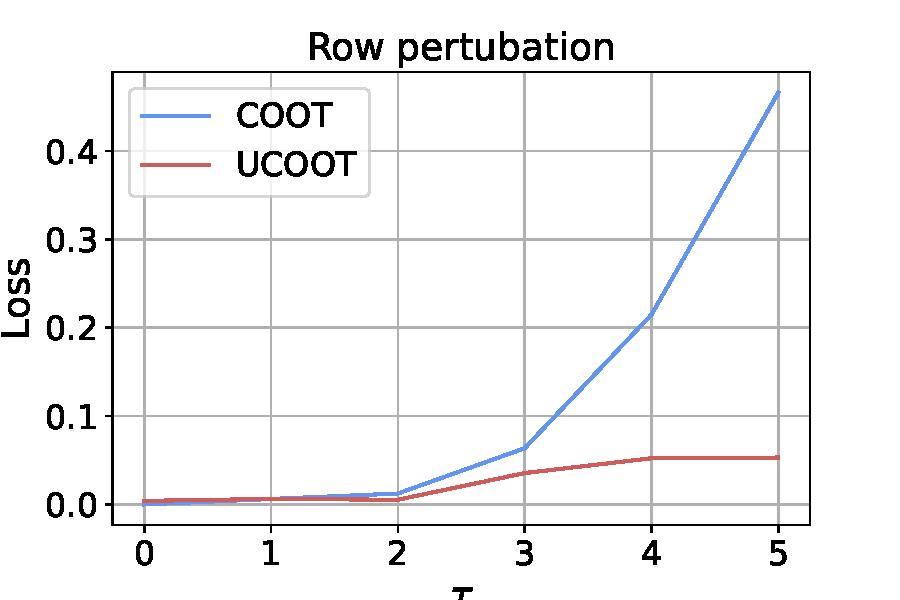
\includegraphics[width=\linewidth]{./Chapitre3/fig/robustness_2.pdf}
  \caption{Sensitivity of COOT and UCOOT under the presence of outliers.
  \label{fig:robust}}
% \end{figure}
\end{wrapfigure}
This is well illustrated in \Cref{fig:robust},
where we simulate outliers by adding a perturbation to a row of the interaction matrix.
More precisely, we first generate a matrix $A \in \mathbb R^{20 \times 15}$ by
$A_{ij} = \cos(\frac{i}{20} \pi) + \cos(\frac{j}{15} \pi)$.
Then, we replace its last row by $\tau \mathds 1_{15}$, for $\tau \geq 0$.
\Cref{fig:robust} depicts COOT and UCOOT between $A$
and its modified version as a function of $\tau$. The higher the value of $\tau$,
the more likely that the last row contains the interaction of outliers.
Consequently, as $\tau$ increases, so does COOT but at a much higher pace,
whereas UCOOT remains stable.

It should be noted that, with minimal adaptation, \Cref{thm:ucoot_robust}
also holds for the unbalanced GW (UGW) distance.
This provides a theoretical explanation of the empirical observation in \citep{Sejourne20}
that unlike GW, the UGW distance is also robust to outliers.

%%%%%%%%%%%%%%%%%%%%%%%%%%%%%%%%%%%%%%%%%%%%%%%%
\section{Optimization algorithm and complexity}
%%%%%%%%%%%%%%%%%%%%%%%%%%%%%%%%%%%%%%%%%%%%%%%%
Solving COOT-type problems, in general, is not trivial. As highlighted in \citep{Redko20},
the balanced case corresponds to a convex relaxation of the bilinear assignment problem,
which seeks the pair of permutations minimizing the transport cost.
Here we argue that relaxing the marginal constraints makes the problem easier
in two different aspects: (1) the obtained problem is easier to solve
through a sequence of GPU friendly iterations; (2) regularization leads to lower alignment costs
and thus better local minima. In this section, we first describe how to compute UCOOT in practice.

\paragraph{Optimization strategy.}
We consider two tabular datasets $A \in \bbR^{n_1 \times d_1}$ and $B \in \bbR^{n_2 \times d_2}$.
Let $u_k$ be the uniform histogram over sample-feature pairs:
$u_k := \frac{1}{n_kd_k}\mathds 1_{n_k} \otimes \mathds 1_{d_k}$, for $k=1, 2$.
For the sake of simplicity, we assume uniform weights over both samples and features.
Computing UCOOT can be done using block-coordinate descent (BCD) both with
and without entropy regularization. More precisely, given a hyperparameter $\varepsilon \geq 0$,
discrete UCOOT can be written as:
\begin{equation}
\begin{split}
    \label{eq:ucoot-discrete-2}
  &\min_{\substack{\pi^s, \pi^f \\
  \iffalse \in \bbR_+^{n_1, n_2} \\ \pi^f \in \bbR_+^{d_1, d_2} \\ \fi m(\pi^s) = m(\pi^f)}}
  \sum_{i, j, k, l} (A_{ik} - B_{jl})^2\pi^s_{ij}\pi^f_{kl} +
  \lambda_1 \kl(\pi^s \mathds 1_{n_1} \otimes \pi^f \mathds 1_{d_1} | u_1 )  \\
  &+ \lambda_2 \kl({\pi^s}^\top \mathds 1_{n_2} \otimes {\pi^f}^{\top} \mathds 1_{d_2} | u_2) +
  \varepsilon \text{KL}( \pi^s \otimes \pi^f | \mu^s_1 \otimes \mu_2^s \otimes \mu_1^f \otimes \mu_2^f).
\end{split}
\end{equation}

\begin{algorithm}
    \caption{BCD algorithm to solve UCOOT \label{alg:bcd}}
    \begin{algorithmic}
      \STATE {\bfseries Input:} $A \in \bbR^{n_1, d_1}, B \in \bbR^{n_2, d_2}$, $\lambda_1, \lambda_2, \varepsilon$
      \STATE Initialize $\pi^s$ and $\pi^f$
      \REPEAT
      \STATE Update $\pi^s$ using Sinkhorn or NNPR
      \STATE Rescale $\pi^s = \sqrt{\frac{m(\pi^f)}{m(\pi^s)}} \pi^s$
      \STATE Update $\pi^s$ using Sinkhorn or NNPR
      \STATE Rescale $\pi^f = \sqrt{\frac{m(\pi^s)}{m(\pi^f)}} \pi^f$
      \UNTIL{convergence}
	\end{algorithmic}
\end{algorithm}
% where recall that the total transported mass $m(\pi)$ is calculated by $\sum_{ij}\pi_{ij}$. The hyperparameters $\lambda_1$ and $\lambda_2$ implicitly control how much of the ``sample-feature'' mass is transported. \huy{this seems a bit redundant because we will rewrite almost the same formulation in the next paragraph.}

The only difference between $\varepsilon = 0$ and $\varepsilon > 0$
lies in the inner-loop algorithm used to update one of transport plans $(\pi^s, \pi^f)$
while the other one remains fixed. Note that both cases allow for
implementations of a scaling multiplicative algorithm that can be parallelized on GPUs.
%: Sinkhorn's algorithm ($\varepsilon > 0$) or NNPR ($\varepsilon = 0
%$).  The main BCD scheme is summarized in \Cref{alg:bcd}.
% ($\varepsilon > 0$ Sinkhorn's algorithm.}
For $\varepsilon > 0$, updating each transport plan boils down to an entropic UOT problem,
which can be solved efficiently using the unbalanced variant of Sinkhorn's algorithm \citep{Chizat18a}.
The main benefit of entropy regularization is to reduce the number of variables
from $(n_1 \times n_2) + (d_1 \times d_2)$ to $n_1 + n_2 + d_1 + d_2$.
Moreover, by taking $\varepsilon$ sufficiently small, we can recover solutions
close to those in the non-entropic case. We formalize this claim in the following result.
%%%%%%%%%%%%%%%%%%%%%%%%%%%%%%%%%%%%%%%%%%
\begin{proposition}
  \label{convergence_minimiser_unbalanced}
  Let $(\pi_{\varepsilon}^s, \pi_{\varepsilon}^f)$ be an equal-mass solution of the problem
  $\ucoot_{\lambda, \varepsilon}(\cX_1, \cX_2)$. Denote $\mu^s = \mu_1^s \otimes \mu_2^s$
  and $\mu^f = \mu_1^f \otimes \mu_2^f$.
  \begin{enumerate}
    \item When $\varepsilon \to \infty$, we have $\pi_{\varepsilon}^s \rightharpoonup
    \sqrt{\frac{m(\mu^f)}{m(\mu^s)}} \mu^s$
    and $\pi_{\varepsilon}^f \rightharpoonup \sqrt{\frac{m(\mu^s)}{m(\mu^f)}} \mu^f$.

    \item When $\varepsilon \to 0$, we have
    \begin{enumerate}
      \item $\ucoot_{\lambda, \varepsilon}(\cX_1, \cX_2) \to \ucoot_{\lambda}(\cX_1, \cX_2)$ and
      $m(\pi_{\varepsilon}^s) \to m(\pi_*^s)$, for any equal-mass solution
      $(\pi_*^s, \pi_*^f)$ of the unregularized problem.

      \item Any cluster point $(\widehat{\pi}^s, \widehat{\pi}^f)$ of the sequence
      $(\pi_{\varepsilon}^s, \pi_{\varepsilon}^f)_{\varepsilon}$ is an equal-mass
      solution of the unregularized problem. Furthermore,
      \begin{equation}
        \kl(\widehat{\pi}^s \otimes \widehat{\pi}^f | \mu^s \otimes \mu^f) =
        \min_{(\pi^s, \pi^f)} \kl(\pi^s \otimes \pi^f \vert \mu^s \otimes \mu^f),
      \end{equation}
      where the infimum is taken over all solutions of the unregularized problem.
    \end{enumerate}
  \end{enumerate}
\end{proposition}

\iffalse It should also be noted that, while the proposed algorithm in \citep{Sejourne21}
requires mass rescaling within each BCD iteration, it is not necessarily the case for the UCOOT. \fi
For $\varepsilon=0$, the non-regularized UOT problem can be recast as a
non-negative penalized regression (NNPR)~\citep{Chapel21}.
This problem can be solved using a majorization-minimization algorithm
which leads to a multiplicative update on the transport plan.
\iffalse The NNPR was proposed and extensively studied by \citep{Chapel21}. \fi
For the sake of reproducibility, we provide the details on the optimization scheme
of both algorithms in the Appendix.

\section{Experiments} \label{sec:experiments}
\subsection{Illustration and interpretation on MNIST images}

\begin{figure}[t]
  \centering
  \includegraphics[trim={0.5cm 4.5cm 1.5cm 2.4cm}, clip, width=\linewidth]{./Chapitre3/fig/mnist-ucoot-rebuttal.pdf}
  \caption{Example illustrating the feature alignment $\pi_f$ learned by UCOOT
  and its robustness to outliers.
  \textbf{(a)} Visualization of 4 random samples from both datasets.
  The added Gaussian noise only affects the first 10 columns of the images
  and is different across images.
  \textbf{(b)} The barycentric mapping (see Appendix for details)
  defined by UCOOT learns the transformation defined by $\varphi_\sigma$
  while disregarding non-informative features.
  \textbf{(c)} Alignments across samples from $X$ and $Y$.
  We contaminated the target $Y$ with 50 sample outliers
  (images with uniform entries in $[0,1]$).
  A very small amount of noise is sufficient to derail COOT.
  Unlike COOT, UCOOT does not transport any outlier sample.
  Accuracy is computed as the percentage of mass within the block-diagonal structure.
  \label{f:mnist-example}}
\end{figure}
We illustrate the robustness of UCOOT and its ability to learn meaningful feature alignments
under the presence of both sample and feature outliers in the MNIST dataset.
We introduce the feature outliers by applying a handcrafted transformation $\varphi_\sigma$
that performs a zero-padding (shift), a 45\textdegree\ rotation,
a resize to (28, 34) and adds Gaussian noise $\cN(0, \sigma^2)$ entries
to the first 10 columns of the image.

\Cref{f:mnist-example} (a) shows some examples of original and transformed images.
We randomly sample 100 images per class (1000 total) from $X = \text{MNIST}$ and
$Y = \varphi_{\sigma}(\text{MNIST})$. Regarding the sample outliers,
we add 50 random images with uniform entries in [0, 1] to the target data $Y$.
We then compute the optimal COOT and UCOOT alignments shown in
\Cref{f:mnist-example} (b) and (c).
The flexibility of UCOOT with respect to mass transportation allows it to completely disregard:
(1) noisy and uninformative pixels (features),
which are all given the same weight as depicted by (b);
(2) all the sample outliers of which none are transported as shown
by the last blank column of the alignment (c).
Moreover, notice how the color-coded input image is transformed according to
the transformation $\varphi_{\sigma}$ despite the fact that
no spatial information is provided in the OT problem. On the other hand,
a very small perturbation ($\sigma = 0.01)$ is enough for the sample alignment
given by COOT to lose its block-diagonal dominant structure (class information is lost),
while the UCOOT alignment remains unscathed.

\setlength{\intextsep}{0pt}
\begin{wrapfigure}[10]{r}{0.4\textwidth}
  % \begin{figure}
    \centering
    \vspace{-12pt}
    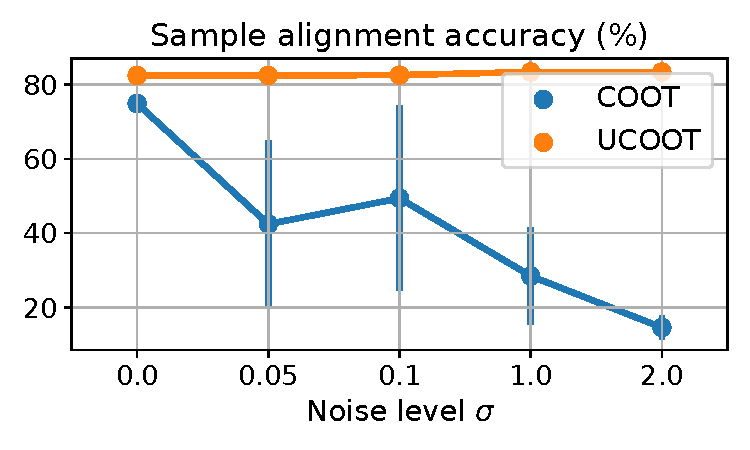
\includegraphics[width=\linewidth]{./Chapitre3/fig/mnist-sigma.pdf}
    \vspace*{-9mm}
    \caption{Robustness of UCOOT vs. COOT on MNIST example, at different noise levels.
    \label{f:mnist-sigma}}
  % \end{figure}
\end{wrapfigure}
One may wonder whether the performance of UCOOT would still hold for different values of $\sigma$.
\Cref{f:mnist-sigma} answers this question positively.
For $\sigma > 0$, we compute the average accuracy
(defined by the percentage of mass within the block-diagonal structure) over 20 different runs.
The performance of COOT not only degrades with noisier outliers but is also unstable.
By contrast, the accuracy of UCOOT remains almost constant regardless of the level of noise.

\subsection{Heterogeneous Domain Adaptation}

%Domain adaptation (DA) refers to the problem in which a classifier
%learned on one domain (called \textit{source}) can generalise well to the other one (called \textit{target}).
We now investigate the application of discrete UCOOT in semi-supervised and unsupervised
Heterogeneous Domain Adaptation (HDA). It is a particularly difficult problem where
one aims to predict classes on unlabeled data using labeled data lying in a different space.
OT methods across spaces have recently shown good performance on such tasks,
in particular using GW distance ~\citep{Yan18} and COOT~\citep{Redko20}.
%i.e. the samples in source and target domains live in the different spaces, and we have no access to the labelled target sample.
%It should be noted that COOT and UCOOT have already been used in real-world applications.
% For example, as the entropic GW distance and its COOT follow exactly the same approximation scheme, they share the success in
% graph matching \citep{Xu19b}, correspondance alignment \citep{Solomon16},
% comparing kernel matrices \citep{peyre16}. On the other hand, the recent discrete COOT also works well in co-clustering and
% HDA tasks \citep{Redko20} and the UCOOT has shown competitive performance in positive-unlabelled learning \citep{Sejourne20}.

\paragraph{Datasets and experimental setup.} We consider the Caltech-Office dataset~\citep{Saenko10}
containing three domains:
Amazon (A) ($1123$ images), Caltech-$256$ (C) ($958$ images) and Webcam (W) ($295$ images)
with 10 overlapping classes amongst them. The image in each domain is representated by
the output of the second last layer
in the Google Net~\citep{Szegedy15} and Caffe Net~\citep{Jia14} neural network architectures,
which results in $4096$ and $1024$-dimensional vectors, respectively (thus $d_s = 4096, d_t = 1024$).
We compare $4$ OT-based methods: GW, COOT, UGW, and UCOOT. For the semi-supervised HDA task,
we additionally use $k$-NN, with $k=3$ as baseline method, which corresponds to the situation where
there is no adaptation. The hyper-parameters for each method are validated on a
unique pair of datasets (W$\rightarrow$W),
then fixed for all other pairs in order to provide truly unsupervised HDA generalization.

We follow the same experimental setup as in \citep{Redko20}. For each pair of domains,
we randomly choose $20$ samples per class (thus $n_s = n_t = 200$) and
perform adaptation from CaffeNet to GoogleNet features, then calculate the
accuracy of the generated predictions on the target domain using OT label propagation \citep{Redko19a}.
This technique uses the OT plan to estimate the amount of mass transported from each class
(since the sources are labeled) to a given target sample.
The predicted class corresponds to the one which contains the most mass.
% : except for the baseline, for each method, we use the learned sample coupling between source and
% target data to predict the labels in the target domain via label propagation \citep{Redko19a}.
% More precisely, for each pair of domains, we randomly choose $20$ samples per class (thus $n_s = n_t = 200$) and
% perform adaptation from CaffeNet to GoogleNet features, then calculate the accuracy of the generated predictions on the target domain.
We repeat this process $10$ times and calculate the average and standard deviation of the performance.
In both source and target domains, we assign uniform sample and feature distributions.

In the semi-supervised HDA task, we incorporate the prior knowledge on the target labels by adding an
additional cost matrix to the training of sample coupling, so that a source sample
will be penalized if it transfers mass to the target samples in the different classes.
More precisely, we introduce the masked target label $\tilde{y}^{(t)} \in \mathbb R^{n_t}$
defined by randomly keeping $\tilde{n}_t \in \{1,3,5\}$ samples in each class
in the target label $y^{(t)}$ and masking all other labels in $y^{(t)}$ by $-1$.
Then the additional cost $M \in \mathbb R^{n_s \times n_t}$ between $y^{(s)}$
and $\tilde{y}^{(t)}$ is defined by
\begin{equation}
  M_{ij} =
  \begin{cases}
    0, \text{ if } y^{(s)}_i = \tilde{y}^{(t)}_j, \text{ or } \tilde{y}^{(t)}_j = -1 \\
    v, \text{ otherwise}.
  \end{cases}
\end{equation}
Here, $v > 0$ is a fixed value and we choose $v = 100$ in this experiment.

Once the sample coupling $P$ is learned, the label propagation works as follows:
suppose the labels contain $K$ different classes,
we apply the one-hot encoding to the source label $y^{(s)}$ to obtain
$D^{(s)} \in \mathbb R^{K \times n_s}$ where $D^{(s)}_{ki} = 1_{\{y^{(s)}_i = k\}}$.
The label proportions on the target data are estimated by:
$L = D^{(s)} P \in \mathbb R^{K \times n_t}$. Then the prediction can be generated by choosing the
label with the highest proportion, i.e. $\widehat{y}^{(t)}_j = \arg\max_k L_{kj}$.
Note that, while the prediction is performed on the whole target samples,
only those whose labels are masked as $-1$ during the
training, are used in the calculation of accuracy. For the $k$-NN only,
we train a classifier on the labelled target samples, then perform prediction on the unlabelled ones.

\paragraph{HDA results.}
\begin{table}[t]
  \centering
  \small
		\begin{tabular}{c c c c c}
				\toprule
				Domains & GW & UGW & COOT & UCOOT \\
				\midrule

				C $\to$ C & 16.25 ($\pm$ 7.54) & 10.85 ($\pm$ 2.13) & 36.40 ($\pm$ 12.94) & \textbf{44.05 ($\pm$ 19.33)} \\
				\hline
				C $\to$ A & 12.95 ($\pm$ 7.74) & 11.60 ($\pm$ 4.86) & 28.30 ($\pm$ 11.78) & \textbf{31.90 ($\pm$ 7.43)} \\
				\hline
				C $\to$ W & 18.95 ($\pm$ 9.43) & 14.15 ($\pm$ 3.98) & 19.55 ($\pm$ 14.51) & \textbf{28.55 ($\pm$ 6.60)} \\
				\hline

				A $\to$ C & 16.40 ($\pm$ 8.99) & 10.25 ($\pm$ 5.66) & \textbf{41.80 ($\pm$ 14.81)} & 39.15 ($\pm$ 17.98) \\
				\hline
				A $\to$ A & 14.75 ($\pm$ 15.20) & 20.20 ($\pm$ 6.45) & \textbf{57.90 ($\pm$ 16.84)} & 42.45 ($\pm$ 15.47) \\
				\hline
				A $\to$ W & 14.55 ($\pm$ 8.83) & 20.65 ($\pm$ 4.13) & 42.10 ($\pm$ 7.80) & \textbf{48.55 ($\pm$ 13.06)} \\
				\hline

				W $\to$ C & 20.65 ($\pm$ 11.90) & 14.20 ($\pm$ 5.13) & 8.60 ($\pm$ 6.56) & \textbf{69.80 ($\pm$ 14.91)} \\
				\hline
				W $\to$ A & 17.00 ($\pm$ 9.75) & 7.10 ($\pm$ 2.45) & 16.65 ($\pm$ 10.01) & \textbf{30.55 ($\pm$ 10.09)} \\
				\hline
				W $\to$ W & 19.30 ($\pm$ 11.87) & 24.40 ($\pm$ 3.28) & \textbf{75.30 ($\pm$ 3.26)} & 51.50 ($\pm$ 20.51) \\
				\bottomrule
				Average & 16.76 ($\pm$ 10.14) & 14.82 ($\pm$ 4.23) & 36.29 ($\pm$ 10.95) & \textbf{42.94 ($\pm$ 13.93)} \\
				\bottomrule
			\end{tabular}
	\caption{Unsupervised HDA from CaffeNet to GoogleNet. \label{tab:hda}}
\end{table}

The means and standard deviations of the accuracy on target data are reported in \Cref{tab:hda}
for all the methods and all pairs of datasets. We observe that, thanks to its robustness,
UCOOT outperforms COOT on 7 out of 9 dataset pairs, with higher average accuracy
but also slightly larger variance. This is because of the difficulty of the
unsupervised HDA problem and the instability present in all methods. In particular,
GW-based approaches perform very poorly. This may be due to the fact that the
pre-trained models contain meaningful but a very high-dimensional vectorial representation
of the image. Thus, using the Euclidean distance matrices as inputs not only causes
information loss but also is less relevant (see for example, \citep{Aggarwal01},
or Theorem 3.1.1 and Remark 3.1.2 in \citep{Vershynin18}).

\begin{table}[t]
  \small
  \centering
  \begin{tabular}{c c c c c c}
    \toprule
    Domains & Baseline & GW & UGW & COOT & UCOOT \\
    \midrule
    & \multicolumn{4}{c}{\large{$\tilde{n}_t = 1$}} \\
    \midrule

    C $\to$ C & 28.32 ($\pm$ 6.28) & 35.37 ($\pm$ 8.85) & 29.21 ($\pm$ 6.54) & \textbf{87.37 ($\pm$ 2.90)} & 85.00 ($\pm$ 2.03) \\
    \hline
    C $\to$ A & 25.32 ($\pm$ 9.61) & 31.47 ($\pm$ 8.76) & 26.84 ($\pm$ 7.93) & 85.42 ($\pm$ 6.21) & \textbf{85.79 ($\pm$ 6.19)} \\
    \hline
    C $\to$ W & 30.05 ($\pm$ 5.90) & 42.53 ($\pm$ 6.31) & 40.47 ($\pm$ 8.32) & 64.68 ($\pm$ 7.88) & \textbf{67.00 ($\pm$ 8.80)} \\
    \hline

    A $\to$ C & 39.63 ($\pm$ 7.21) & 36.11 ($\pm$ 8.04) & 29.47 ($\pm$ 5.50) & 80.74 ($\pm$ 9.87) & \textbf{84.11 ($\pm$ 8.34)} \\
    \hline
    A $\to$ A & 42.21 ($\pm$ 7.60) & 37.84 ($\pm$ 16.34) & 39.11 ($\pm$ 11.56) & 93.42 ($\pm$ 1.32) & \textbf{93.58 ($\pm$ 1.12)} \\
    \hline
    A $\to$ W & 36.21 ($\pm$ 9.45) & 43.58 ($\pm$ 3.75) & 52.21 ($\pm$ 8.26) & \textbf{91.63 ($\pm$ 2.57)} & 90.37 ($\pm$ 6.51) \\
    \hline

    W $\to$ C & 30.16 ($\pm$ 7.22) & 40.68 ($\pm$ 8.11) & 32.63 ($\pm$ 7.70) & 78.84 ($\pm$ 4.24) & \textbf{79.05 ($\pm$ 3.81)} \\
    \hline
    W $\to$ A & 31.89 ($\pm$ 6.55) & 42.37 ($\pm$ 7.35) & 26.26 ($\pm$ 4.67) & \textbf{95.84 ($\pm$ 2.51)} & 89.37 ($\pm$ 11.34) \\
    \hline
    W $\to$ W & 24.16 ($\pm$ 6.79) & 43.89 ($\pm$ 4.64) & 44.00 ($\pm$ 5.10) & 96.58 ($\pm$ 5.54) & \textbf{98.00 ($\pm$ 2.04)} \\
    \midrule
    Average & 32.57 ($\pm$ 7.72) & 39.32 ($\pm$ 8.02) & 35.58 ($\pm$ 7.29) & \textbf{86.06 ($\pm$ 4.78)} & \underline{85.81 ($\pm$ 5.58)} \\

    \midrule
    & \multicolumn{4}{c}{\large{$\tilde{n}_t = 3$}} \\
    \midrule

    C $\to$ C & 65.82 ($\pm$ 4.28) & 39.41 ($\pm$ 9.83) & 45.41 ($\pm$ 5.56) & 87.18 ($\pm$ 2.05) & \textbf{87.76 ($\pm$ 2.10)} \\
    \hline
    C $\to$ A & 68.06 ($\pm$ 5.89) & 46.24 ($\pm$ 10.45) & 54.94 ($\pm$ 7.29) & \textbf{86.94 ($\pm$ 3.18)} & 85.53 ($\pm$ 3.13) \\
    \hline
    C $\to$ W & 69.94 ($\pm$ 4.92) & 44.12 ($\pm$ 4.99) & 52.71 ($\pm$ 6.25) & \textbf{83.76 ($\pm$ 2.22)} & 83.41 ($\pm$ 5.60) \\
    \hline

    A $\to$ C & 82.88 ($\pm$ 4.44) & 51.29 ($\pm$ 3.71) & 48.71 ($\pm$ 6.10) & 90.12 ($\pm$ 1.76) & \textbf{90.18 ($\pm$ 3.18)} \\
    \hline
    A $\to$ A & 81.88 ($\pm$ 4.13) & 84.41 ($\pm$ 4.69) & 74.00 ($\pm$ 6.73) & 93.59 ($\pm$ 1.91) & \textbf{94.65 ($\pm$ 1.69)} \\
    \hline
    A $\to$ W & 84.76 ($\pm$ 2.91) & 57.76 ($\pm$ 9.23) & 59.35 ($\pm$ 4.20) & \textbf{93.82 ($\pm$ 1.75)} & 93.59 ($\pm$ 1.40) \\
    \hline

    W $\to$ C & 83.06 ($\pm$ 4.75) & 51.94 ($\pm$ 8.68) & 58.24 ($\pm$ 2.44) & \textbf{95.76 ($\pm$ 2.17)} & 92.71 ($\pm$ 6.19) \\
    \hline
    W $\to$ A & 82.12 ($\pm$ 3.69) & 66.41 ($\pm$ 10.75) & 69.53 ($\pm$ 5.62) & 97.12 ($\pm$ 0.61) & \textbf{97.71 ($\pm$ 0.61)} \\
    \hline
    W $\to$ W & 80.41 ($\pm$ 3.56) & 66.82 ($\pm$ 3.26) & 69.06 ($\pm$ 5.39) & 99.24 ($\pm$ 0.75) & \textbf{99.41 ($\pm$ 0.53)} \\
    \midrule
    Average & 77.18 ($\pm$ 3.91) & 56.49 ($\pm$ 7.29) & 59.11 ($\pm$ 5.51) & \textbf{91.95 ($\pm$ 1.82)} & \underline{91.66 ($\pm$ 2.71)} \\

    \midrule
    & \multicolumn{4}{c}{\large{$\tilde{n}_t = 5$}} \\
    \midrule

    C $\to$ C & 71.60 ($\pm$ 4.12) & 50.67 ($\pm$ 3.78) & 53.07 ($\pm$ 4.68) & 86.07 ($\pm$ 2.36) & \textbf{87.53 ($\pm$ 2.09)} \\
    \hline
    C $\to$ A & 73.80 ($\pm$ 3.14) & 62.80 ($\pm$ 5.16) & 64.87 ($\pm$ 3.78) & 86.40 ($\pm$ 2.62) & \textbf{86.60 ($\pm$ 2.72)} \\
    \hline
    C $\to$ W & 72.53 ($\pm$ 4.13) & 57.27 ($\pm$ 2.74) & 57.07 ($\pm$ 4.08) & \textbf{88.20 ($\pm$ 2.07)} & 85.13 ($\pm$ 4.28) \\
    \hline

    A $\to$ C & 86.20 ($\pm$ 3.07) & 52.07 ($\pm$ 3.16) & 50.67 ($\pm$ 4.32) & 91.47 ($\pm$ 2.12) & \textbf{93.87 ($\pm$ 1.81)} \\
    \hline
    A $\to$ A & 88.73 ($\pm$ 2.66) & 71.93 ($\pm$ 5.50) & 74.80 ($\pm$ 7.84) & 93.53 ($\pm$ 1.71) & \textbf{94.13 ($\pm$ 1.54)} \\
    \hline
    A $\to$ W & 88.80 ($\pm$ 2.60) & 67.47 ($\pm$ 5.26) & 66.07 ($\pm$ 5.66) & \textbf{93.13 ($\pm$ 2.19)} & \textbf{93.13 ($\pm$ 1.79)} \\
    \hline

    W $\to$ C & 91.33 ($\pm$ 2.49) & 59.33 ($\pm$ 4.15) & 54.73 ($\pm$ 3.68) & \textbf{95.87 ($\pm$ 1.63)} & 95.47 ($\pm$ 1.90) \\
    \hline
    W $\to$ A & 90.93 ($\pm$ 3.40) & 68.13 ($\pm$ 4.01) & 70.53 ($\pm$ 3.71) & 97.53 ($\pm$ 1.27) & \textbf{98.73 ($\pm$ 0.63)} \\
    \hline
    W $\to$ W & 91.47 ($\pm$ 3.40) & 68.67 ($\pm$ 3.71) & 72.93 ($\pm$ 3.17) & \textbf{99.40 ($\pm$ 0.63)} & \textbf{99.40 ($\pm$ 0.47)} \\
    \bottomrule
    Average & 83.84 ($\pm$ 3.43) & 62.04 ($\pm$ 4.16) & 62.75 ($\pm$ 4.55) & \underline{92.40 ($\pm$ 1.84)} & \textbf{92.67 ($\pm$ 1.91)} \\
    \bottomrule
  \end{tabular}
  \caption{Semi-supervised HDA from CaffeNet to GoogleNet, for different values of $\tilde{n}_t$.}
  \label{tab:table2}
\end{table}
However, under the presence of
labelled target samples, \Cref{tab:table2} shows that the advantage of UCOOT diminishes significantly,
as the level of certainty increases. In this case, both COOT and UCOOT
are also much more stable but UCOOT is somewhat more volatile than COOT.

\paragraph{Robustness to target shift.}
We also illustrate the robustness of UCOOT to a change in class proportions,
also known as target shift.

\begin{wrapfigure}[10]{r}{0.4\textwidth}
  \centering
  \vspace{-10pt}
  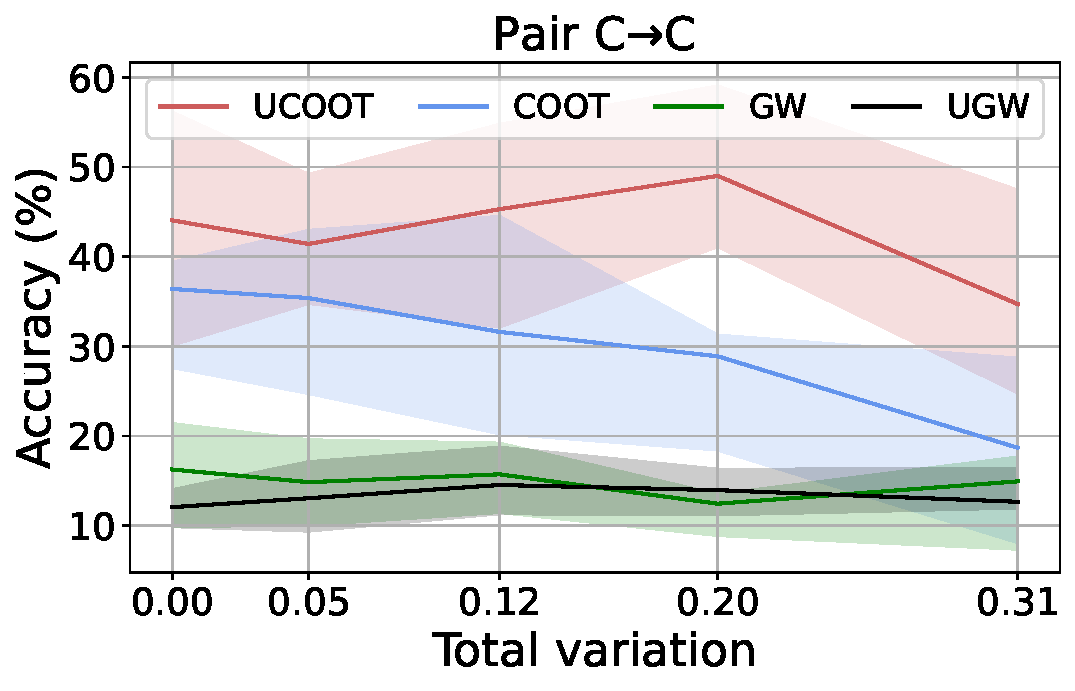
\includegraphics[width=\linewidth]{./Chapitre3/fig/summary_C_C.pdf}
  \vspace*{-7mm}
  \caption{Robustness to class proportion change for increasing TV on the class marginals.
  \label{f:hda_prop}}
\end{wrapfigure}
More precisely, we simulate a change in proportion only in the source domain
by selecting $20\rho$ samples per class for 4 amongst 10 classes with $\rho$
decreasing from $\rho=1$ to $\rho=0.2$. In this configuration,
the classes in the source domain are imbalanced and the unlabeled HDA problem becomes more difficult.
We report the performance of all the methods as a function of the Total Variation (TV)
between the class marginal distributions on one pair of datasets in \Cref{f:hda_prop}.
We can see that UCOOT is quite robust to change in class proportions,
while COOT experiences a sharp decrease in accuracy when the class distributions
become more imbalanced.

% We observe that in general, UCOOT is less stable than COOT, due to the mass
% relaxation nature. This is advantageous in the unsupervised HDA tasks, where, in absence of
% target labels, this relaxation provides flexibility to deals with the uncertainty of labels.
% For this reason, UCOOT usually outperforms COOT by large margins.
%
%\paragraph{Robustness to target shift}
\subsection{Single-cell multi-omics alignment}
Finally, we present a real-world application of UCOOT for the alignment of single-cell measurements.
Recent advances in single-cell sequencing technologies allow biologists to measure
a variety of cellular features at the single-cell resolution, such as expression levels of genes
and epigenomic changes in the genome \citep{Buenrostro15,Chen19},
or the abundance of surface proteins \citep{CITEseq}. These multiple measurements produce
single-cell multi-omics datasets. These datasets measuring different biological phenomena
at the single-cell resolution allow scientists to study how the cellular processes are regulated,
leading to finer cell variations during development and diseases. However, it is hard to obtain
multiple types of measurements from the same individual cells due to experimental limitations.
Therefore, many single-cell multi-omics datasets have disparate measurements from different
sets of cells. As a result, computational methods are required to align the cells and
the features of the different measurements to learn the relationships between them that help
with data analysis and integration. Multiple tools \citep{Pamona, Seurat, Liu2019},
including GW \citep{Pamona, Demetci22} and UGW \citep{Demetci22-2} based methods,
have shown good performance for cell-to-cell alignments.
% However,  aligning both samples and features is a more challenging and critical task for this domain that can be solved by the UCOOT formulation.
However, aligning both samples and features is a more challenging and critical task that
GW and UGW-based methods cannot address
%\pinar{since they compute alignments between intra-domain distances, discarding features \citep{Demetci22, Pamona, Demetci22-2}}.
Here we provide an application of UCOOT to simultaneously align the samples and features
in a single-cell multi-omics dataset.
%
%how the features in different molecular features relate to one another.
%As a result, we require computational methods to align the cells and the features of the different measurements to obtain correspondence between similar cells and features. This correspondence information can help investigate which features in one domain (e.g., genes) match the ones (e.g., proteins) in the other domain.
%

\begin{figure}
    \centering
    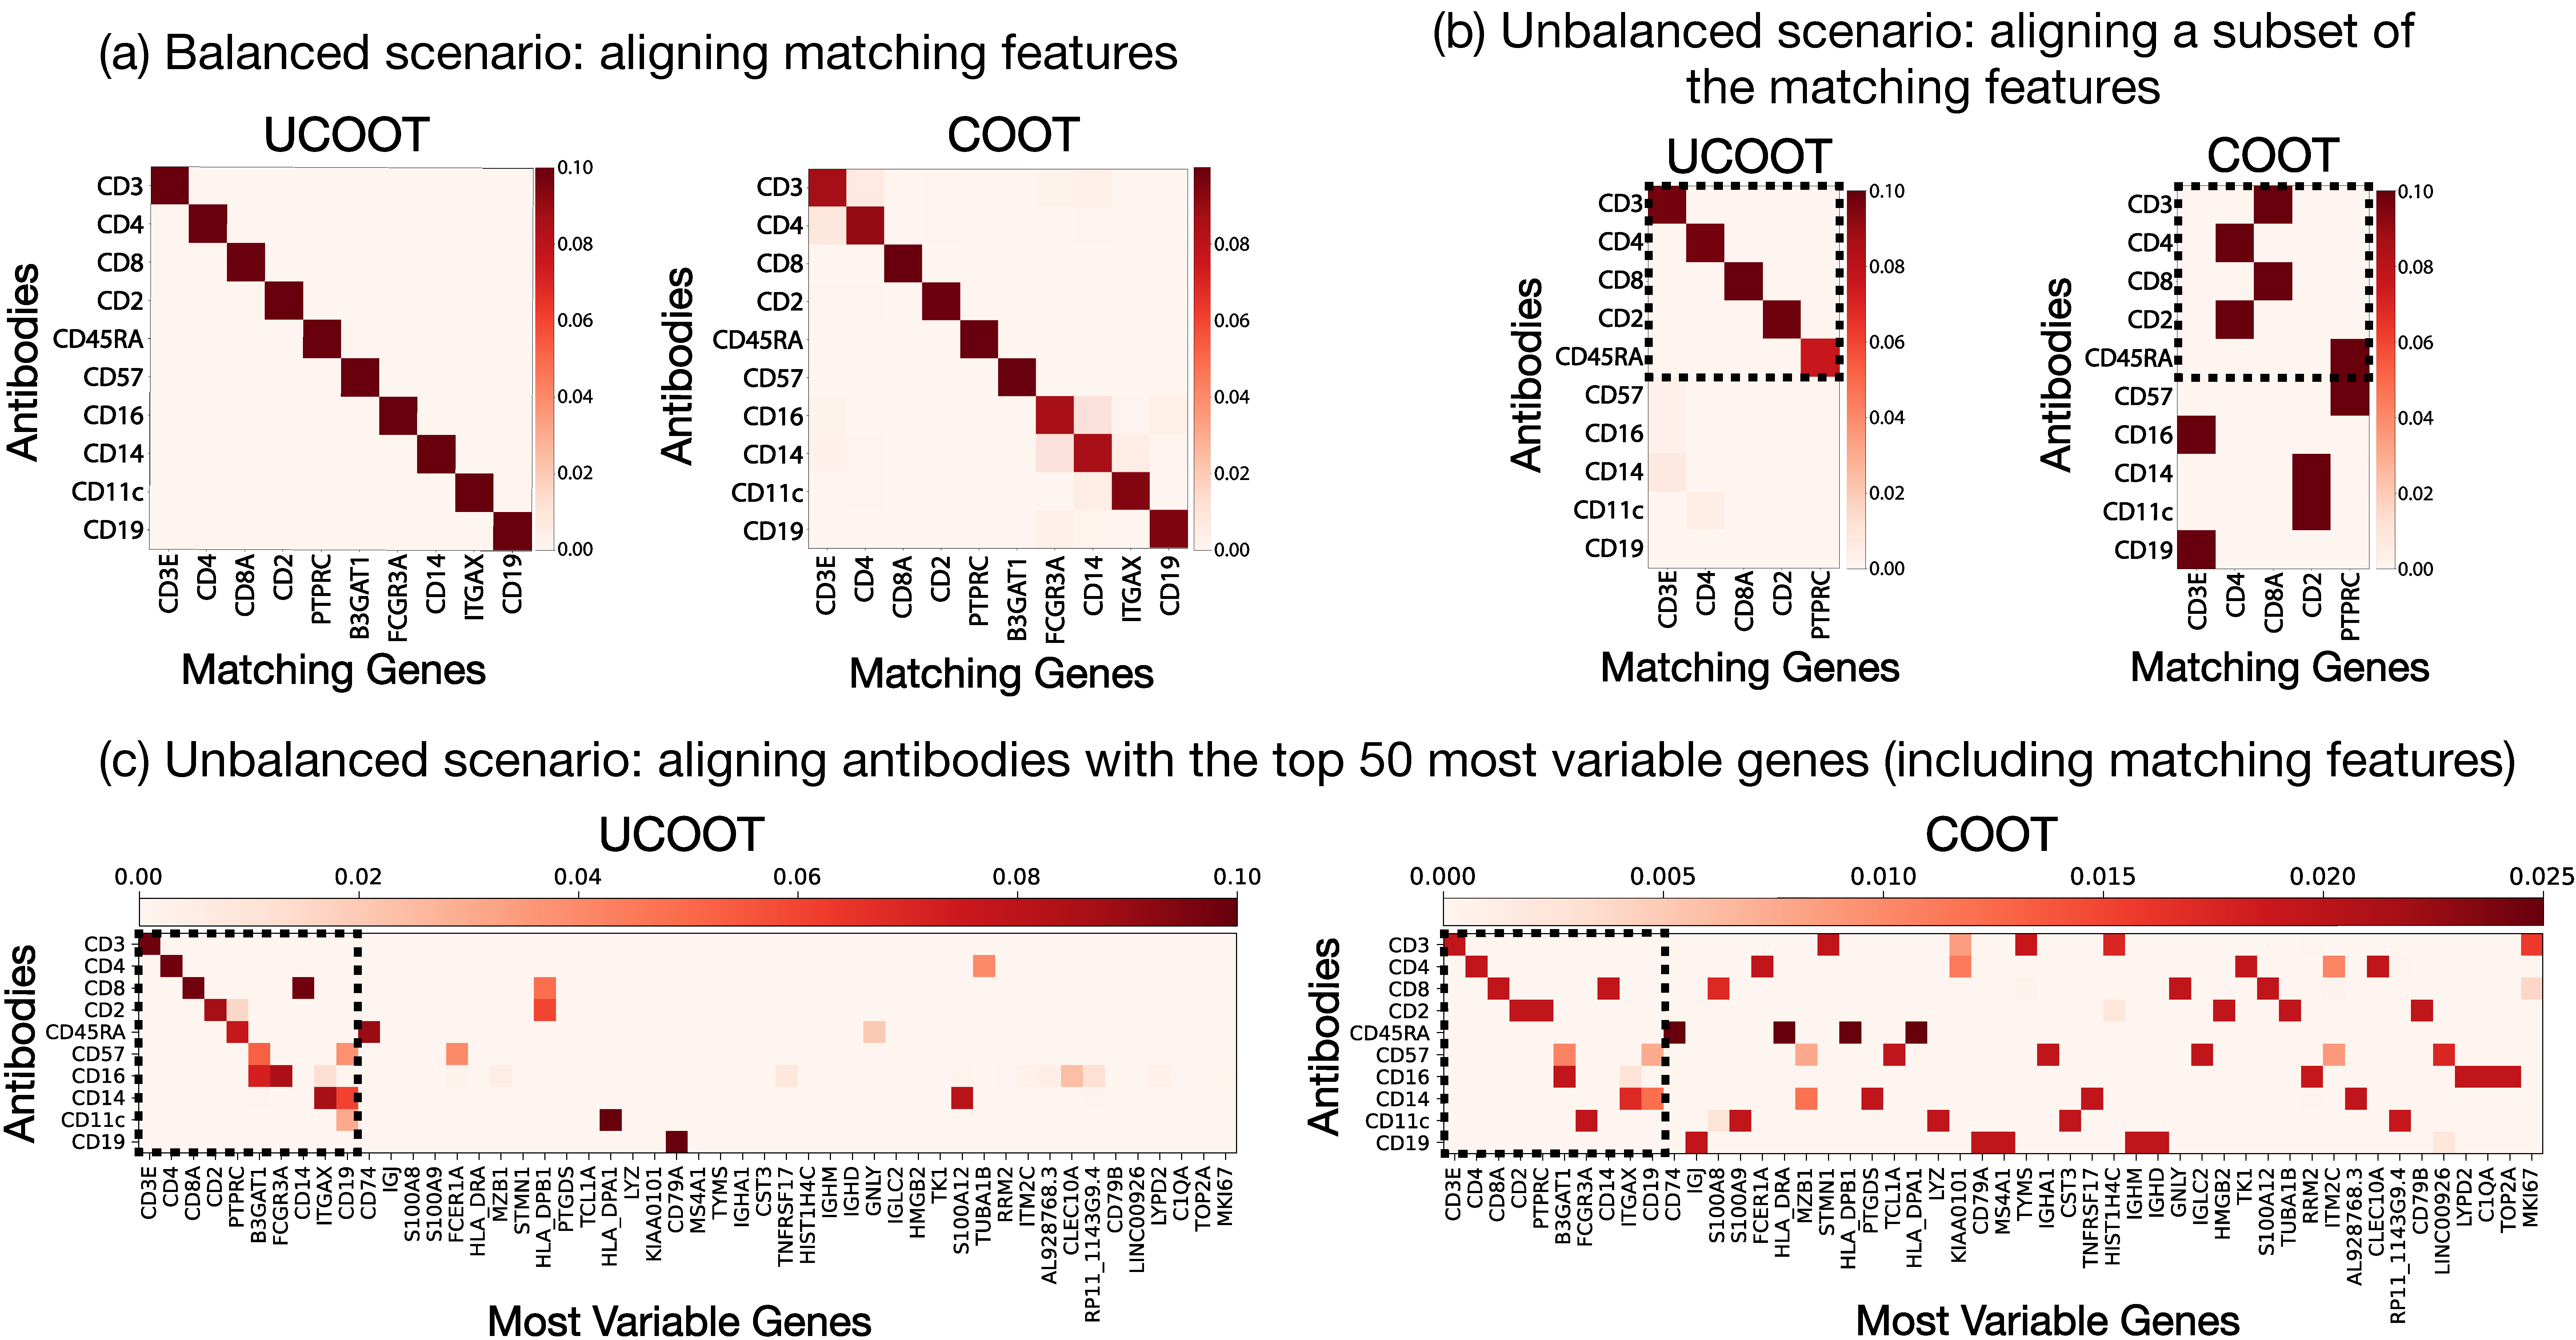
\includegraphics[trim={0.2cm 0.2cm 0.8cm 0.5cm}, clip, width=\linewidth, keepaspectratio=true]{./Chapitre3/fig/genes-alignments.pdf}
    \caption{Feature alignments on the single-cell multi-omics dataset of COOT and UCOOT between antibodies (surface proteins) and their matching genes (that encode them). \textbf{(a)} The features are sorted such that the correct alignment would yield a diagonal matrix. \textbf{(b)} Only five of the correct gene matches are kept (the last five genes from (a) are excluded). \textbf{(c)} Alignments between the ten antibodies and the top 50 most variable genes, including the matching genes.
    For \textbf{(b)} and \textbf{(c)}, the diagonal within the dashed square highlights the correct matches.
    Overall, UCOOT gives better feature alignments.
    \label{fig:multiomics}}
\end{figure}

For demonstration, we choose a dataset generated by the CITE-seq experiment \citep{CITEseq},
which simultaneously measures gene expression and antibody (or surface protein)
abundance in single cells. From this dataset, we use 1000 human peripheral blood cells,
which have ten antibodies and 17,014 genes profiled. We selected this specific dataset
as we know the ground-truth correspondences on both the samples (i.e., cells)
and the features (i.e., genes and their encoded antibodies), thus allowing us to quantify
and compare the alignment performance of UCOOT and COOT.
As done previously \citep{Pamona, Demetci22, Liu2019}, we quantify the cell alignment performance
by calculating the fraction of cells closer than the true match (FOSCTTM) of each cell
in the dataset and averaging it across all cells. This metric quantifies alignment error,
so lower values are more desirable. The feature alignments are measured by calculating
the accuracy of correct matching. The results are presented after hyperparameter tuning
both methods with similar grid size per hyperparameter (see Experimental Details in Appendix).

% I'll move the details about the original dataset to the Appendix
% The particular dataset we work with profiles a mix of 7,985 human and mouse peripheral blood mononuclear cells and contains measurements on 10 antibodies, 17014 human genes and 12915 mouse genes. We select 1000 human cells from this dataset to work with.

\textbf{Balanced Scenario.} First, we select and align the same number of samples and features
across the two datasets. For this, we subset the gene expression domain with the ten genes that
match to the ten antibodies they express. Original data contains the same number of cells
across domains since both domains are simultaneously measured in the same single-cells.
We observe that both UCOOT and COOT can correctly align features (\Cref{fig:multiomics}~(a))
and the cells (Appendix Figure S1(a)) across the two measurements. However,
UCOOT gives better performance, as demonstrated by a lower FOCSTTM score (0.0062 vs 0.0127)
for cells. Both COOT and UCOOT recover the diagonal for matching features (100\% accuracy),
but UCOOT recovers the exact matching, likely due to its robustness to noise,
whereas COOT assigns weights to other features as well.

\textbf{Unbalanced Scenarios.} Next, we perform alignment with an unequal number of features.
This setting is more likely to occur for real-world single-cell datasets as different features
are measured. In the first simple scenario, we align the ten antibodies with only a subset (five)
of their matching genes. As visualized in \Cref{fig:multiomics}~(b),
COOT struggles to find the correct feature alignments (60\% accuracy),
which would lie in the diagonal of the highlighted square (dashed lines). However,
the relaxation of the mass conservation constraint in UCOOT allows it to shrink
the mass of antibodies that lack matches in the gene expression domain,
leading do higher accuracy (100\% accuracy).

Next, we align the ten antibodies with
the 50 most variable genes in the dataset, including their matching genes.
This alignment task is the most realistic scenario, as single-cell multi-omics data
consists of high-dimensional datasets with a different number of features for different measurements.
% \pinar{Moreover, many of these genes show consistent expression levels across }
Therefore, biologists focus their analyses on the reduced set of most variable features (e.g. genes).
It is also the most computationally challenging case among all our experiments on this dataset.
Hence, we provide sample-level supervision to both methods by giving a cost penalization matrix
based on the correct sample alignments to the sample alignment computation.
We see in \Cref{fig:multiomics}(c) that in comparison to COOT (50\% accuracy),
UCOOT recovers more of the correct feature alignments (70\% accuracy),
and yields fewer redundant alignments  (for more detail, see Experimental Details in Appendix).
Note that UCOOT avoids incorrect mappings by locally shrinking the mass of the features or samples
that lack correspondences. This avoids subsequent incorrect downstream analysis of
the integration results. This property can also help users to discover rare cell types
by observing the extent of mass relaxation per cell or prune uninformative features in
the single-cell datasets.

%Similarly to the alignment in \Cref{fig:multiomics}(b), this is thanks to the mass shrinkage of the features that lack correspondences. By locally adjusting the mass in transport, UCOOT tends to avoid assigning correspondences to samples or features that lack matches across the aligned domains. With this, UCOOT can help users to detect outliers that can result from experimental artifacts,
%(such as rare cell types or lowly expressed genes that are not captured well by a sequencing technology), prune features or discover rare cell types.}

Lastly, we also consider the case of unequal number of samples across the two measurements.
This case is common in real world single-cell multi-omics datasets that are not
simultaneously measured. Demetci \textit{et al.} \citep{Demetci22-2} have shown that
single-cell alignment methods that do not account for this mismatch yield poor alignment results.
Therefore, we downsample the number of cells in one of the domains by 25\%
and perform alignment with the full set of cells in the other domain (Appendix Figure S1(b \& c)).
We compute the FOSCTTM score for all cells that have a true match in the dataset and
report the average values. UCOOT continues to yield a low FOSCTTM score (0.0081 compared to 0.0062
in the balanced scenario), while COOT shows a larger drop in performance
(0.1342 compared to 0.0127 in the balanced scenario).

\section{Discussion and conclusion}
\label{sec:conclusion}

In this work, we present an extension of COOT called unbalanced COOT,
where the hard constraint on the marginal distributions is replaced by a soft control via
the KL divergence. The resulting problem not only benefits from the flexibility of COOT
but also enjoys the provable robustness property under the presence of outliers,
which is not the case for COOT. The experimental results confirm our findings,
yielding a very competitive performance in the unsupervised HDA task, as well as
meaningful feature couplings for the single-cell multi-omics alignment. Also,
while UCOOT introduces additional hyper-parameters, domain knowledge can help narrow down
the range of feasible values, thus reducing the time and computational cost of the tuning process.
Further investigation should be carried out to fully understand and assess
the observed efficiency of UCOOT in real-world applications,
and also explore the possibilities of UCOOT in more diverse applicative settings,
including its use as a loss in deep learning architectures.
Lastly, from a theoretical perspective, statistical properties such as
sample complexity or stability analysis are needed to better understand
the intricate relations between the two sample and feature couplings.
%Future works may also focus on justifying how the relaxation of marginal constraints allows to cope with the class imbalance and provides empirically better initialization to the approximation scheme of COOT, as observed in the experiments. Last but not least, it is interesting to study the connection with the unbalanced GW distance, since in practice, it is estimated using its lower bound, which is in fact a special of UCOOT.

